\documentclass[UTF8]{ctexart}
\usepackage{amsmath}
\usepackage{geometry}
\usepackage{graphicx}
\usepackage{gensymb}
\usepackage{wrapfig}
\usepackage{titlesec}
\usepackage{float}
\geometry{a4paper,scale=0.8}
\title{2020年电磁场与波试题}
\author{Deschain}
\titlespacing*{\section}
{0pt}{0pt}{0pt}
\titlespacing*{\subsection}
{0pt}{0pt}{0pt}
\titlespacing*{\paragraph}
{0pt}{0pt}{0pt}
\titlespacing*{\subparagraph}
{0pt}{0pt}{0pt}
\begin{document}
\maketitle
\section{}
\begin{wrapfigure}{r}{3cm}
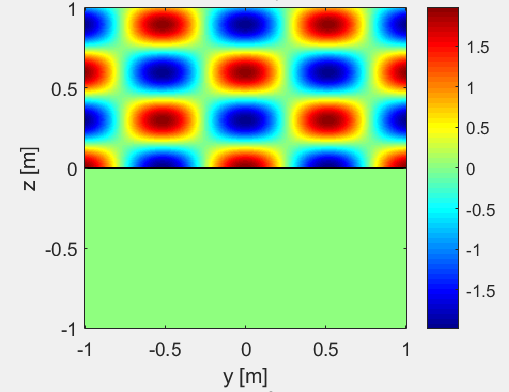
\includegraphics[width=3cm]{2020-1.png}
\end{wrapfigure}
两无限大理想磁壁构成平板波导,全空间$\mu_r=1$,入射波的频率为260MHz,合场沿+y方向传播。在垂直传播方向某场量(x分量)的幅度分布如右图所示。
\subsection{}
请问这是TE波还是TM波?并说明理由。(5分)\\
TE波。在磁壁上存在切向分量,说明垂直方向的场是电场。
\subsection{}
求解介质的相对介电常数。(5分)
\begin{equation*}
\begin{aligned}
&\lambda_z=0.6m,k_z=\frac{2\pi}{\lambda_z}\\
&\lambda_y=1m,k_y=\frac{2\pi}{\lambda_y}\\
&k=\sqrt{k_z^2 + k_y^2},k^2=\omega^2\mu \varepsilon=\omega^2\mu_0\varepsilon_r\varepsilon_0\\
&\varepsilon_r=\frac{k^2}{\omega^2\mu_0\varepsilon_0}=5.03
\end{aligned}
\end{equation*}
\subsection{}
请写出该场的所有电场、磁场分量的完整复数表达式(包括波动项、时谐项)。(5分)
\begin{equation*}
\begin{aligned}
&\vec E=\hat xcos(\frac{2\pi}{0.6}z)e^{j(\omega t-ky)}\\
&\vec H=(\hat yjsin(\frac{2\pi}{0.6}z)+\hat zsin(\frac{2\pi}{0.6}z))e^{j(\omega t-ky)}
\end{aligned}
\end{equation*}
\subsection{}
请画出沿y方向半个波长($\pi$)的电场三维场型(用实线)。(5分)
\subsection{}
请在同一张图中画出沿y方向半个波长($\pi$)的磁场三维场型(用虚线)。(5分)
\begin{figure}[H]
\centering
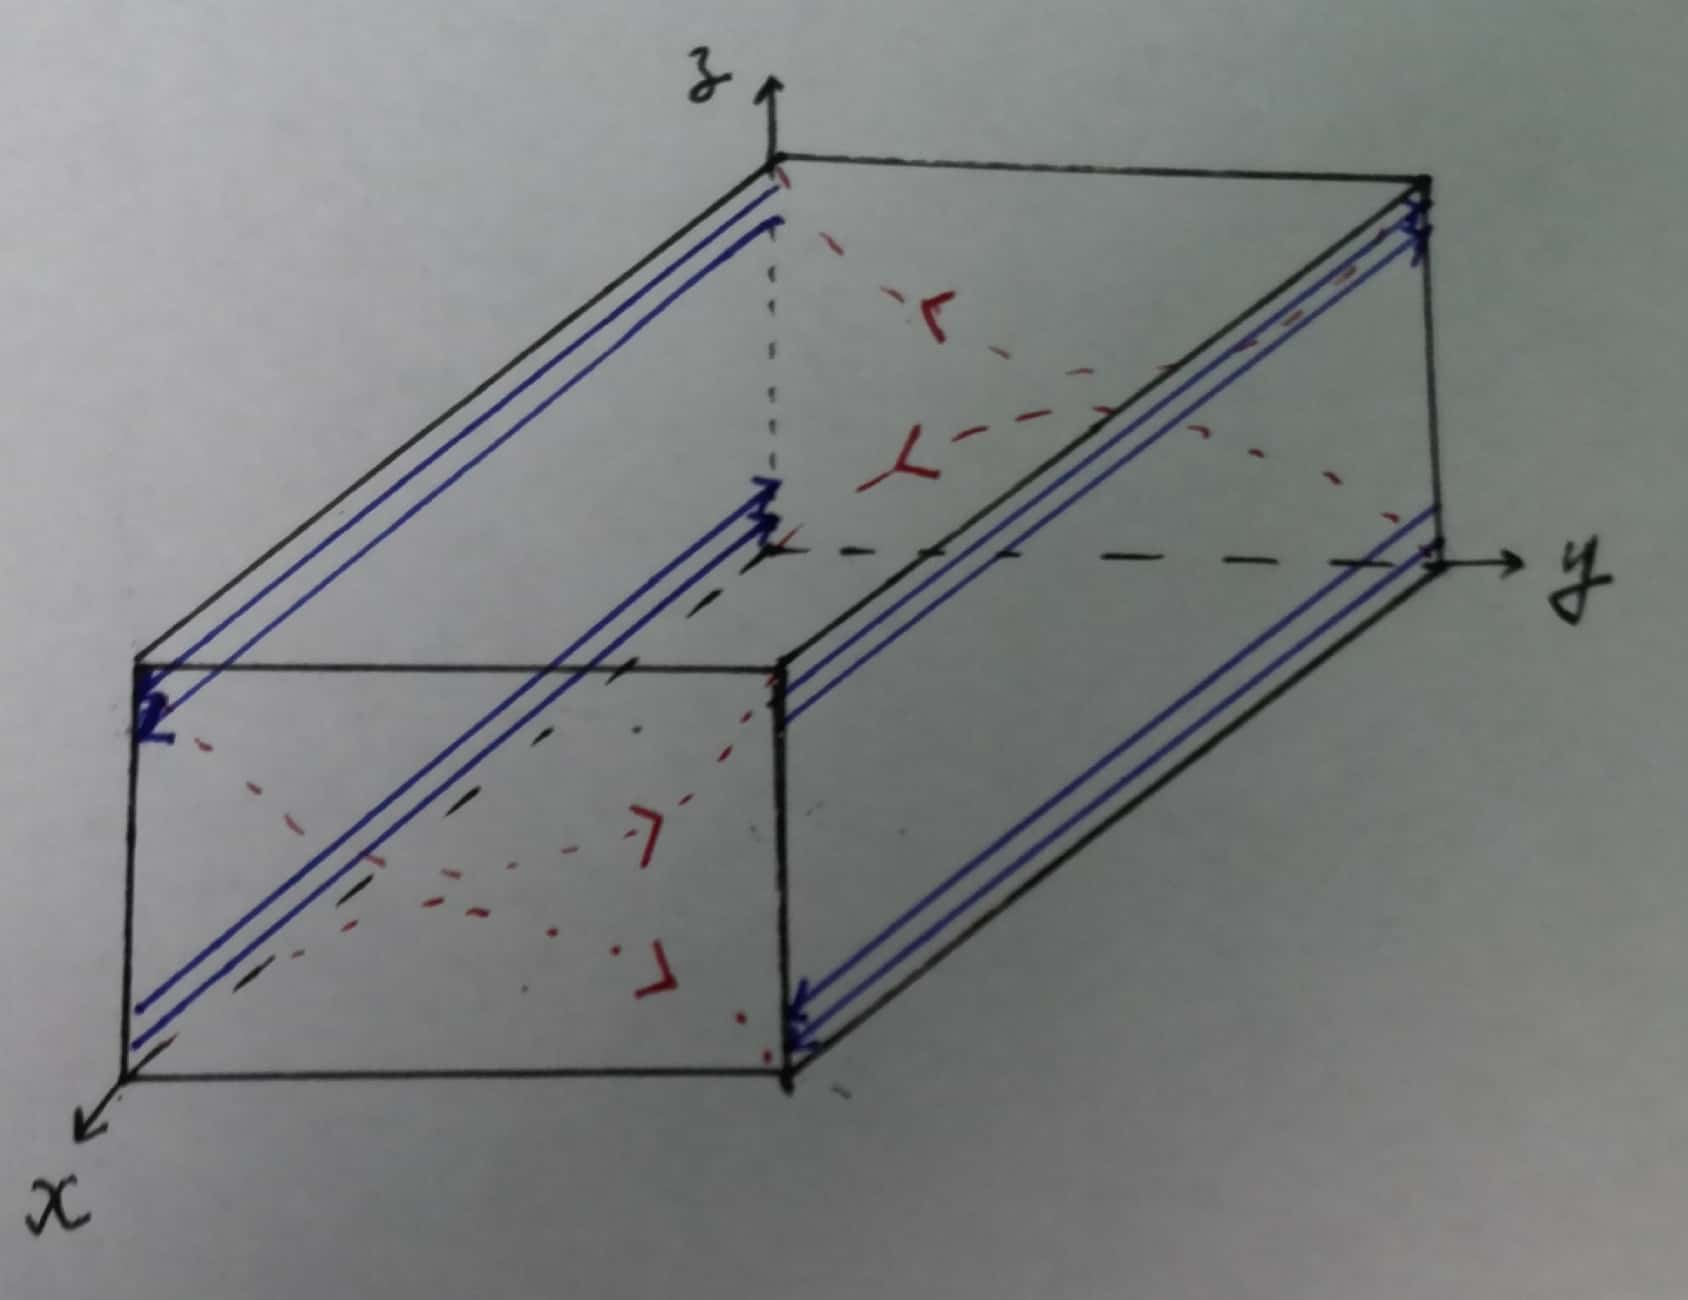
\includegraphics[width=3cm,height=3cm]{2020-2.jpg}
\end{figure}
\section{}
无限大自由空间中
\subsection{静电场}
有一组电荷分布在坐标系原点附近,现需要在-Y轴远离坐标原点的所有位置产生沿$\vec A=\hat\theta+\hat\phi$方向的电场,请给出这组电荷中各电荷的坐标、电场正负与相对电荷量。(5分)\\
(0,0,d):+q\\
(0,0,-d):-q\\
(d,0,0):-q\\
(-d,0,0):+q
\subsection{时变电磁场}
假设辐射源集中在坐标系原点附近,是否可以在-y轴远离坐标原点的所有位置产生沿$\vec A=\hat\theta+\hat\phi$方向的瞬时电场?如果可以,请说明产生方式;如果不可以,请说明原因。(5分)\\
分别沿z轴正向、x轴负向放置两个振荡电偶极子,它们大小相等,相位相同。
\subsection{时变电磁场}
假设辐射源在原点附近,请在球坐标系$(\hat\theta,\hat\phi,\hat r)$下写出-y轴上远离坐标原点的右旋圆极化波的电场的完整复数表达式(包括波动项、时谐项)。(5分)
\[vec E=(\hat\theta-j\hat\phi)e^{j(\omega t-kr)}\]
注:-y轴上的r=-y。
\subsection{时变电磁场}
假设辐射源在原点附近,能否在$\pm X$轴、$\pm Y$轴、$\pm Z$轴上远离原点的所有位置均产生右旋圆极化波?如果能,请说明具体的产生方法;如果不能,请说明理由。(10分)\\
沿z轴正向放置一个电偶极子和一个磁偶极子,两者产生的电场大小相等,电偶极子电场超前磁偶极子电场$\frac{\pi}{2}$。沿y轴正向放置一个电偶极子和一个磁偶极子,两者产生的电场大小相等,电偶极子电场超前磁偶极子电场$\frac{\pi}{2}$。
\section{}
三维柱型区域的静电场边界条件:在Z=0处,$\varphi=0V$;在Z=30处,$\varphi=10V$;在圆柱侧面,$\rho=10$,$(0,\pi)$处$\varphi=10V$;$\rho=10$,$(\pi,2\pi)$处$\varphi=-10V$。
\subsection{}
求区域内电位分布$\varphi(\rho,\phi,z)$的解析表达式,通解的选取需要说明理由。(15分)\\
分解为两个问题。
$\varphi_1$对应于“在Z=30处,$\varphi=10V$,其他边界为0”;$\varphi_1$对应于“$\rho=10$,$(0,\pi)$处$\varphi=10V$;$\rho=10$,$(\pi,2\pi)$处$\varphi=-10V$,其他边界为0”;
\begin{equation*}
\begin{aligned}
&\varphi_1=\sum_{i=1}^{\infty}{AJ_0(k_{zi}z)sh(k_{zi}z)}\\
&\varphi_2=\sum_n^{\infty}\sum_m^{\infty}A_{mn}sin(n\phi)I_n(\frac{m\pi}{30}z)sin(\frac{m\pi}{30}z),\quad\quad n=1,3,5,\cdots
\end{aligned}
\end{equation*}
\subsection{}
现在令Z=30的平面上$\varphi=0V$,取过z轴、y轴的平面,用虚线画出等位线。(5分)
\subsection{}
在同一张图上用实线画出电场线。
\begin{figure}[htbp]
\centering
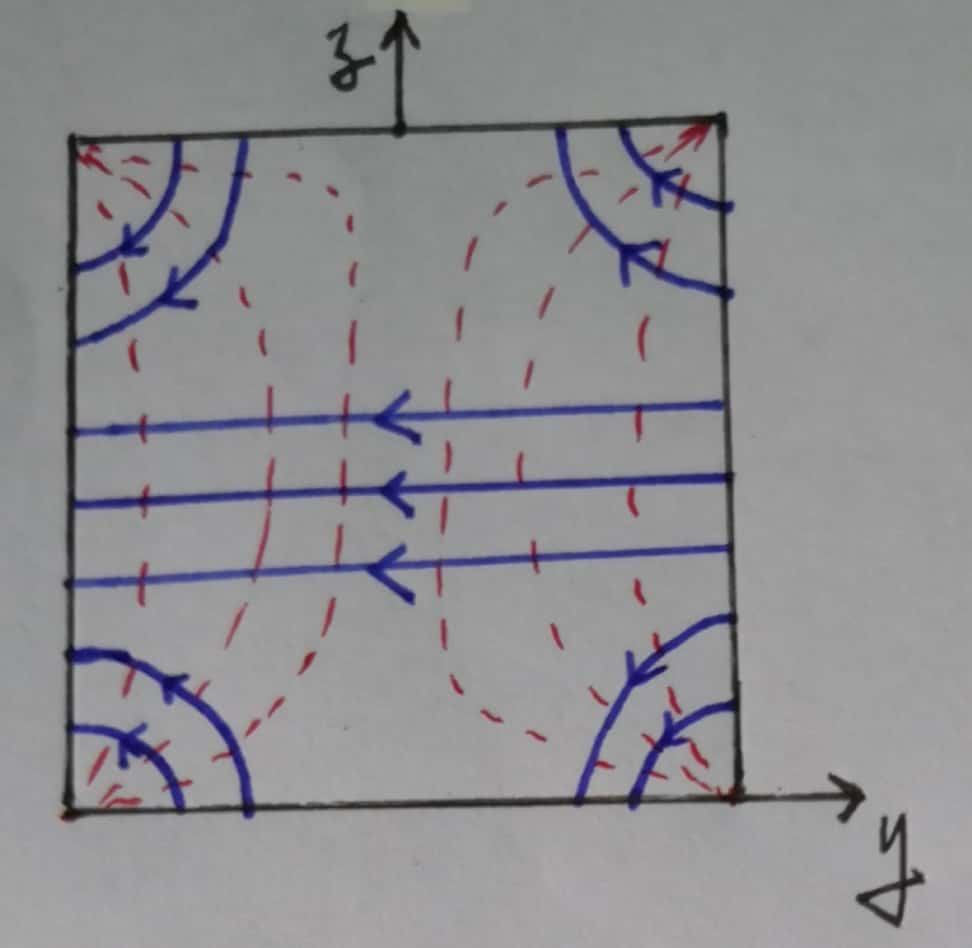
\includegraphics[width=3cm,height=3cm]{2020-3.jpg}
\end{figure}
\section{}
\begin{wrapfigure}{r}{3cm}
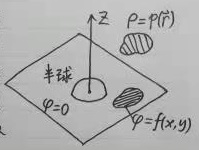
\includegraphics[width=3cm]{2020-4.jpg}
\end{wrapfigure}
考虑如下三维空间,边界由Z=0的无穷大平面和求新在原点、半径为a的半球构成,边界面上,除了S区域满足$\varphi(\vec r)=f(x,y)$,其余均满足$\varphi(\vec r)=0$。在空间中还存在$\rho=\varphi(\vec r)$的电荷分布。
\subsection{}
给出格林函数$G(\vec r,\vec r')$在空间满足的偏微分方程。(5分)
\[\nabla^2G=-\delta(\vec r-\vec r')\]
\subsection{}
请问这是格林函数的第几类边值问题?请给出该格林函数需要满足的边界条件。(5分)
\[G\lvert_{r=a,z>0}=0,\quad G\lvert_{z=0}=0\]
第一类边值问题
\subsection{}
请给出该格林函数的解析解$G(\vec r,\vec r')$。(5分)
\[G(\vec r,\vec r')=\frac{1}{4\pi\varepsilon}(\frac{q}{r_1}-\frac{aq}{dr_2}-\frac{q}{r_3}+\frac{aq}{dr_4})\]
\begin{figure}[htbp]
\centering
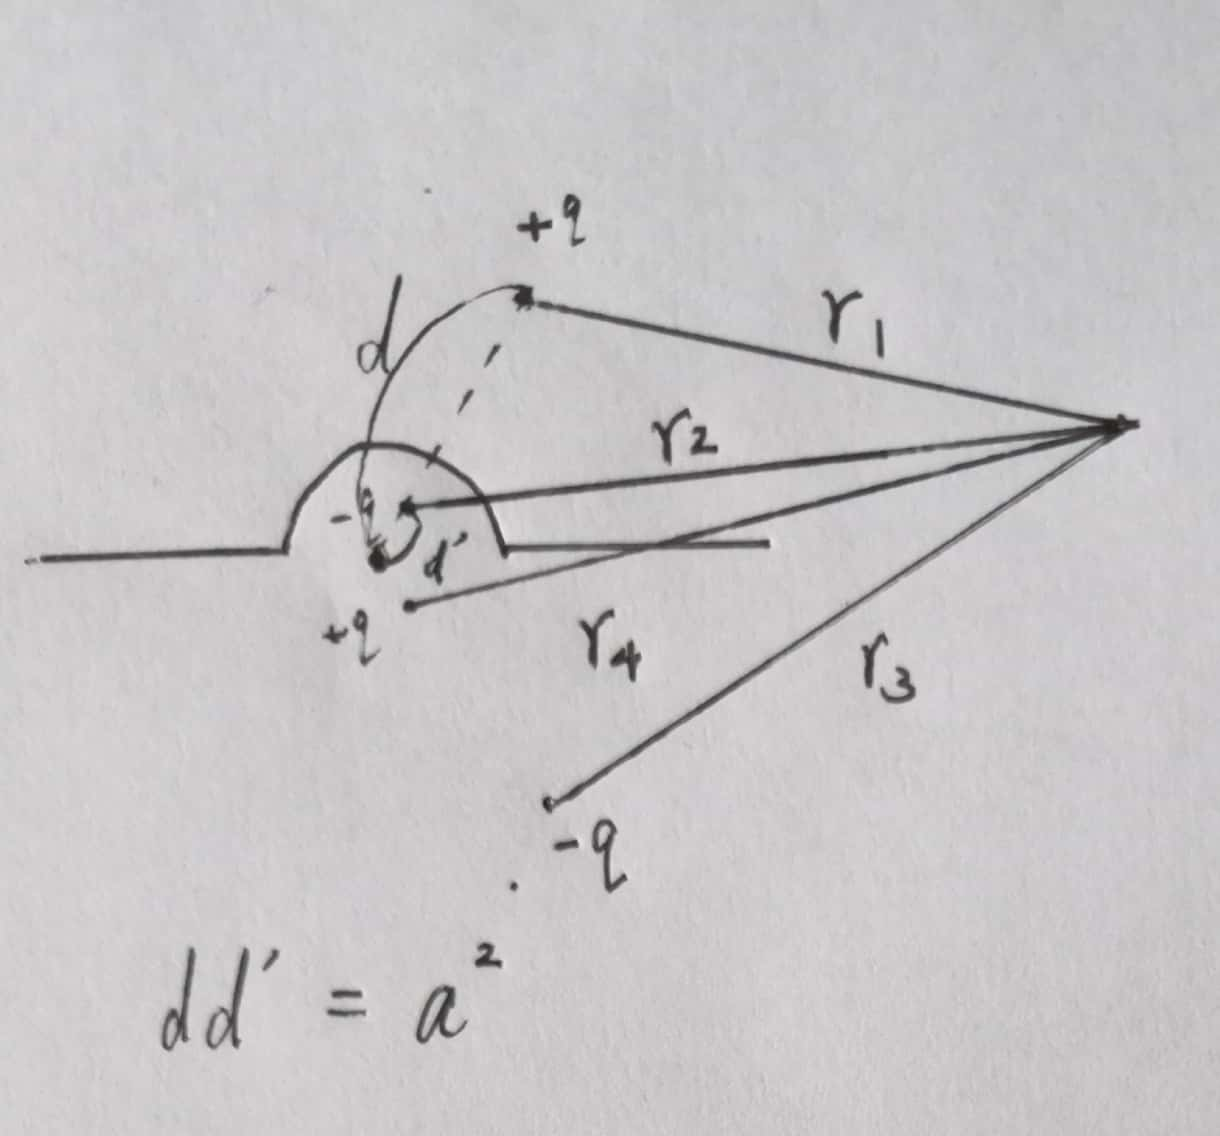
\includegraphics[width=4cm,height=3cm]{2020-5.jpg}
\end{figure}
\subsection{}
请给出化简后的电势积分的格林函数表达式$\varphi(\vec r)=$?(5分)
\[\varphi(\vec r)=\int_V^{}\frac{\rho G}{\varepsilon}dV+\int_S^{}f(x,y)\frac{\partial G}{\partial n}dS\]
V是$\rho=\varphi(\vec r)$存在的区域,S是f(x,y)存在的区域。
\subsection{}
画出该格林函数的梯度场(实线)、等位线(虚线)。绘图面为穿过z轴与源点的平面。
\begin{figure}[H]
\centering
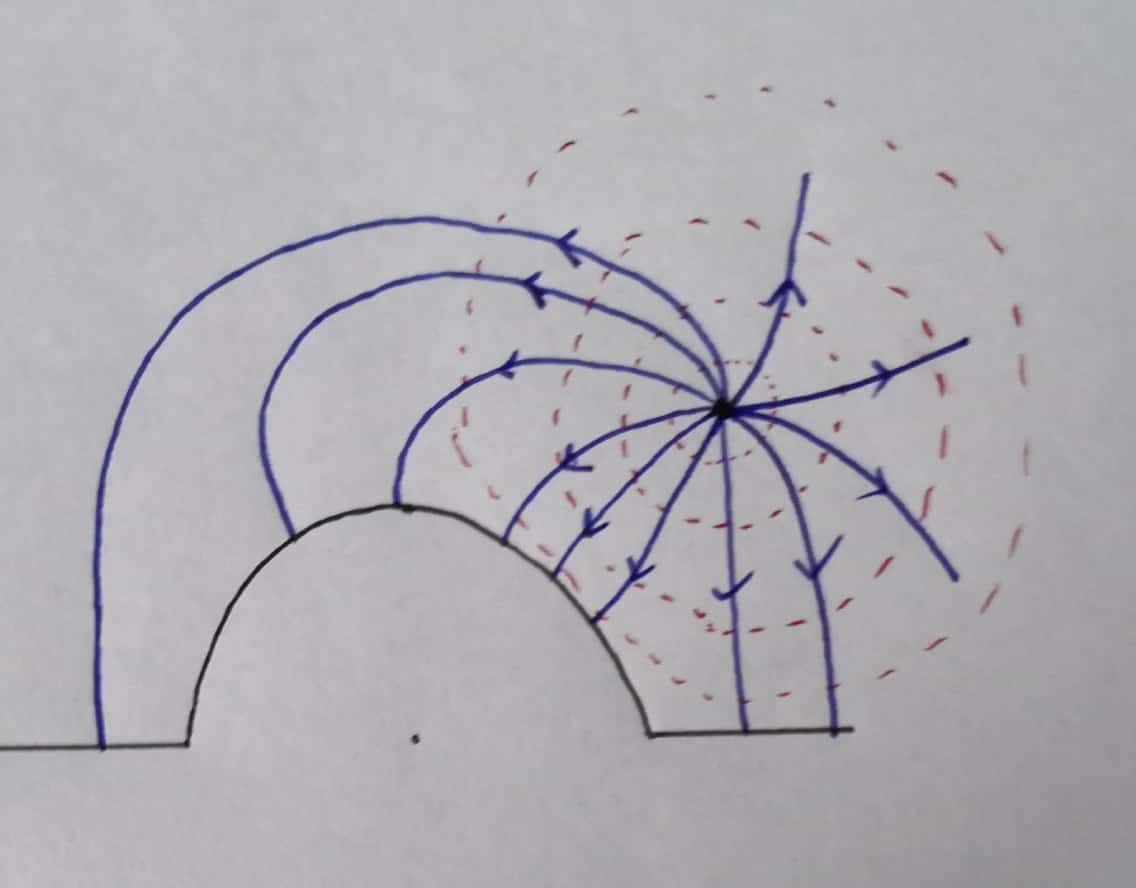
\includegraphics[width=4cm,height=4cm]{2020-6.jpg}
\end{figure}
\end{document}